\chapter{Using the PyCharm IDE}

\setcounter{problem}{1}

\section{Get and install}

\begin{fullwidth}

https://www.jetbrains.com/pycharm/download/

\section{Give it a test drive}

\noindent Create a sample project, making sure that you are using the latest interpreter from homebrew installation ({\tt /usr/local/Cellar/...}):

\scalebox{.75}{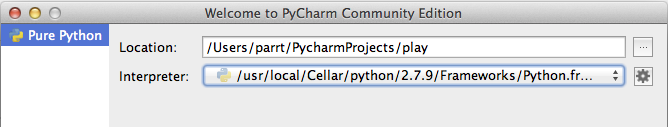
\includegraphics{figures/pycharm-new-project.png}}

\noindent Create a new file with a simple function and run it:

\scalebox{.75}{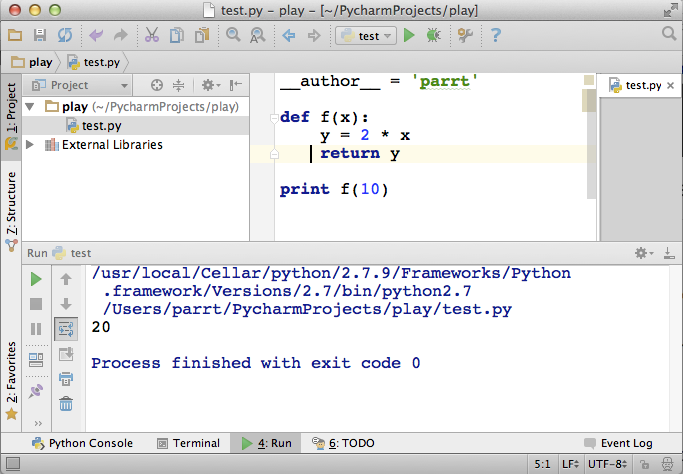
\includegraphics{figures/pycharm-new-file.png}}

\noindent Start up the debugger by clicking the bug icon in the toolbar:

\scalebox{.75}{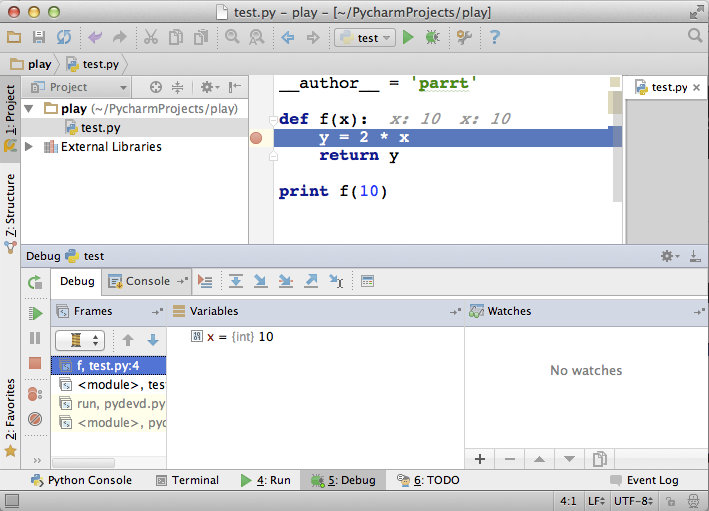
\includegraphics{figures/pycharm-new-dbg.png}}

\noindent Now single step to the next statement:

\scalebox{.75}{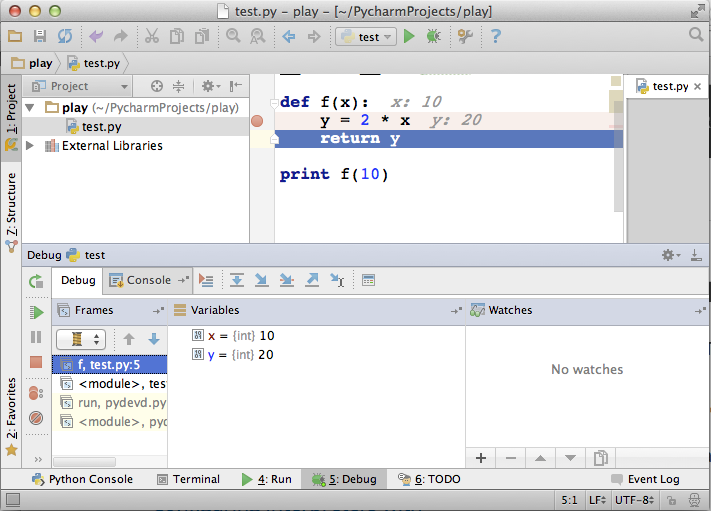
\includegraphics{figures/pycharm-new-dbg2.png}}

\end{fullwidth}
